\documentclass[12pt, letterpaper]{article}

\input{template/preamble.tex}

\input{template/listings_config.tex}

% \input{template/header.tex}

\begin{document}

\begin{titlepage}

	\begin{tikzpicture}[remember picture,overlay]
		\node[anchor=north west, inner sep=30] at (current page.north west) {
			
\includegraphics[width=4cm]{escudoUNAM_color.png}
		};
		% \node[anchor=north west, inner sep=30] at (current page.north west) {
		% 	
\includegraphics[width=4cm]{escudoUNAM_negro.png}
		% };

		\node[anchor=north east, inner sep=30] at (current page.north east) {
			
\includegraphics[width=4cm]{escudoFI_color.png}
		};
		% \node[anchor=north east, inner sep=30] at (current page.north east) {
		% 	
\includegraphics[width=4cm]{escudoFI_negro.png}
		% };
	\end{tikzpicture}

	\begin{center}
		\vspace*{3cm}

		\Huge
		\textbf{Cifrado César}\\

		\vspace{2.5cm}

		\Huge
		\textbf{Facultad de Ingeniería}\\
		Criptografía\\
		\textbf{Dr. Alfonso Francisco de Abiega l'Eglisse} \\
		2027-1\\

		\vspace{2.5cm}

		%grupo de la materia
		\textbf{Grupo:} 3\\

		\vspace{2.5cm}

		\Huge
		Ayala Hernández María Fernanda\\
		López Hernández Miriam Amisadai\\
		Tepal Briseño Hansel Yael\\
		Ugartechea González Luis Antonio\\
		%fecha de entrega
		% \textbf{Fecha de entrega:} <fecha\_entrega>\\
		\vspace{2.5cm}
	\end{center}
\end{titlepage}

\section{Explicación del Cifrado César}

\subsection{Declaración de Variables}

\begin{lstlisting}[style=cstyle, caption={Declaración de variables y arreglos de caracteres.}, label={lst:listing_1}]
char texto[100];
char descifrado[100];
int desplazamiento, valido = 1;
int manual = 0;
\end{lstlisting}

Se declaran los arreglos de caracteres con un límite de 100 espacios para almacenar el mensaje cifrado y el texto descifrado, así como las variables enteras para la llave de cifrado (\texttt{desplazamiento}) y banderas lógicas de control (\texttt{valido} y \texttt{manual}).

\subsection{Selección de la Llave}

\begin{lstlisting}[style=cstyle, caption={Selección de la llave de cifrado.}, label={lst:listing_2}]
    printf("Desea ingresar manualmente la llave de cifrado? (1 para sí, 0 para no): ");
    if (scanf("%d", &manual) != 1) {
        printf("No se pudo leer la opción.\n");
        return 1;
    }
    if (manual) {
        printf("Ingrese la llave de cifrado (0-25): ");
        if (scanf("%d", &desplazamiento) != 1) {
            printf("No se pudo leer la llave.\n");
            return 1;
        }
        if (desplazamiento < 0 || desplazamiento > 25) {
            printf("La llave debe estar entre 0 y 25.\n");
            return 1;
        }
    } else {
        srand((unsigned int)time(NULL));
        desplazamiento = rand() % 26;
    }
\end{lstlisting}

El uso del formato \texttt{\%99[\textasciicircum\textbackslash n]} en \texttt{scanf}nos permite leer hasta 99 caracteres (dejando espacio para el carácter nulo) incluyendo espacios, deteniéndose al encontrar un salto de línea. Posteriormente, se pregunta si la llave se ingresará de manera manual. Si el usuario elige que sí, se lee la llave y se valida que esté en el rango del alfabeto (0 a 25). Si no, se utiliza \texttt{srand} con el tiempo del sistema para inicializar la semilla y se genera un desplazamiento aleatorio usando la operación módulo 26.

Para evitar un cifrado erróneo de símbolos no contemplados, se realiza una iteración sobre la cadena para verificar que todos los caracteres pertenezcan al alfabeto inglés (mayúsculas 'A'-'Z', minúsculas 'a'-'z'). Si se encuentra un carácter que no cumple estas condiciones, la bandera \texttt{valido} se marca como falsa (0), interrumpiendo el bucle y abortando la ejecución con un mensaje de error.

\subsection{Proceso de Cifrado}

\begin{lstlisting}[style=cstyle, caption={Proceso de cifrado del mensaje.}, label={lst:listing_3}]
    for (int i = 0; texto[i] != '\0'; i++) {
        if (texto[i] >= 'A' && texto[i] <= 'Z') {
            texto[i] = (char)('A' + (texto[i] - 'A' + desplazamiento) % 26);
        } else if (texto[i] >= 'a' && texto[i] <= 'z') {
            texto[i] = (char)('a' + (texto[i] - 'a' + desplazamiento) % 26);
        }
    }
\end{lstlisting}

Este fragmento es el la matemática del algoritmo César. Se evalúa cada carácter válido: si es letra, se aplica la fórmula modular \texttt{(caracter - base + desplazamiento) \% 26}. Restar la base ('A' o 'a') mapea la letra al rango numérico de 0 a 25. Luego se suma el desplazamiento y se aplica el módulo 26 para que el conteo regrese a cero si sobrepasa la letra 'Z'. Finalmente, se suma la base ASCII para recuperar el carácter cifrado correspondiente. Los espacios son ignorados intencionalmente y no sufren mutación.

\subsection{Proceso de Descifrado}

\begin{lstlisting}[style=cstyle, caption={Proceso de descifrado del mensaje.}, label={lst:listing_4}]
    for (int i = 0; descifrado[i] != '\0'; i++) {
        if (descifrado[i] >= 'A' && descifrado[i] <= 'Z') {
            descifrado[i] = (char)('A' + (descifrado[i] - 'A' - desplazamiento + 26) % 26);
        } else if (descifrado[i] >= 'a' && descifrado[i] <= 'z') {
            descifrado[i] = (char)('a' + (descifrado[i] - 'a' - desplazamiento + 26) % 26);
        }
    }
\end{lstlisting}

Primero, el mensaje que ha sido cifrado en el propio arreglo \texttt{texto} se copia al arreglo \texttt{descifrado}, cuidando de copiar progresivamente el carácter nulo \texttt{'\textbackslash 0'} para delimitar correctamente el string. El proceso de descifrado es equivalente al cifrado pero a la inversa: se resta el desplazamiento. Como en el lenguaje C la operación módulo de números negativos puede arrojar un resultado negativo, se le suma 26 previamente, garantizando que \texttt{\% 26} siempre devuelva un índice positivo dentro del alfabeto.

\subsection{Salida de Resultados}

\begin{lstlisting}[style=cstyle, caption={Salida de resultados del programa.}, label={lst:listing_5}]
    printf("Llave generada: %d\n", desplazamiento);
    printf("Mensaje cifrado: %s\n", texto);
    printf("Mensaje descifrado: %s\n", descifrado);

    return 0;
\end{lstlisting}

El programa concluye imprimiendo en pantalla la llave numérica utilizada (lo cual es vital si fue generada mediante el modo aleatorio), la cadena resultante del cifrado y la cadena tras someterse al proceso de descifrado.

\subsection{Salida en terminal}

\begin{figure}[H]
    \centering
    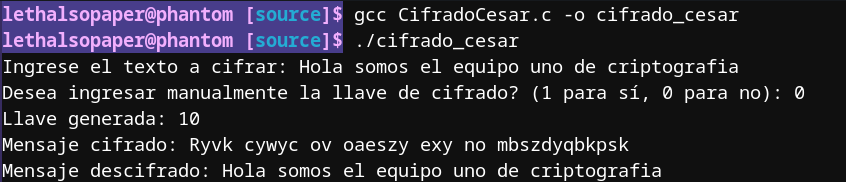
\includegraphics[width=0.8\textwidth]{img/ejemplo_terminal.png}
    \caption{Ejemplo de salida en terminal.}
    \label{fig:ejemplo_terminal}
\end{figure}

\subsection{Repositorio y Código Fuente}

\textbf{Link del repositorio:} \url{https://github.com/HansMarcus01/Criptografia-2027-1}

\textbf{Código fuente:} \url{}

% \input{template/biblio.tex}

\end{document}
